\begin{figure*}[p]
    \centering
    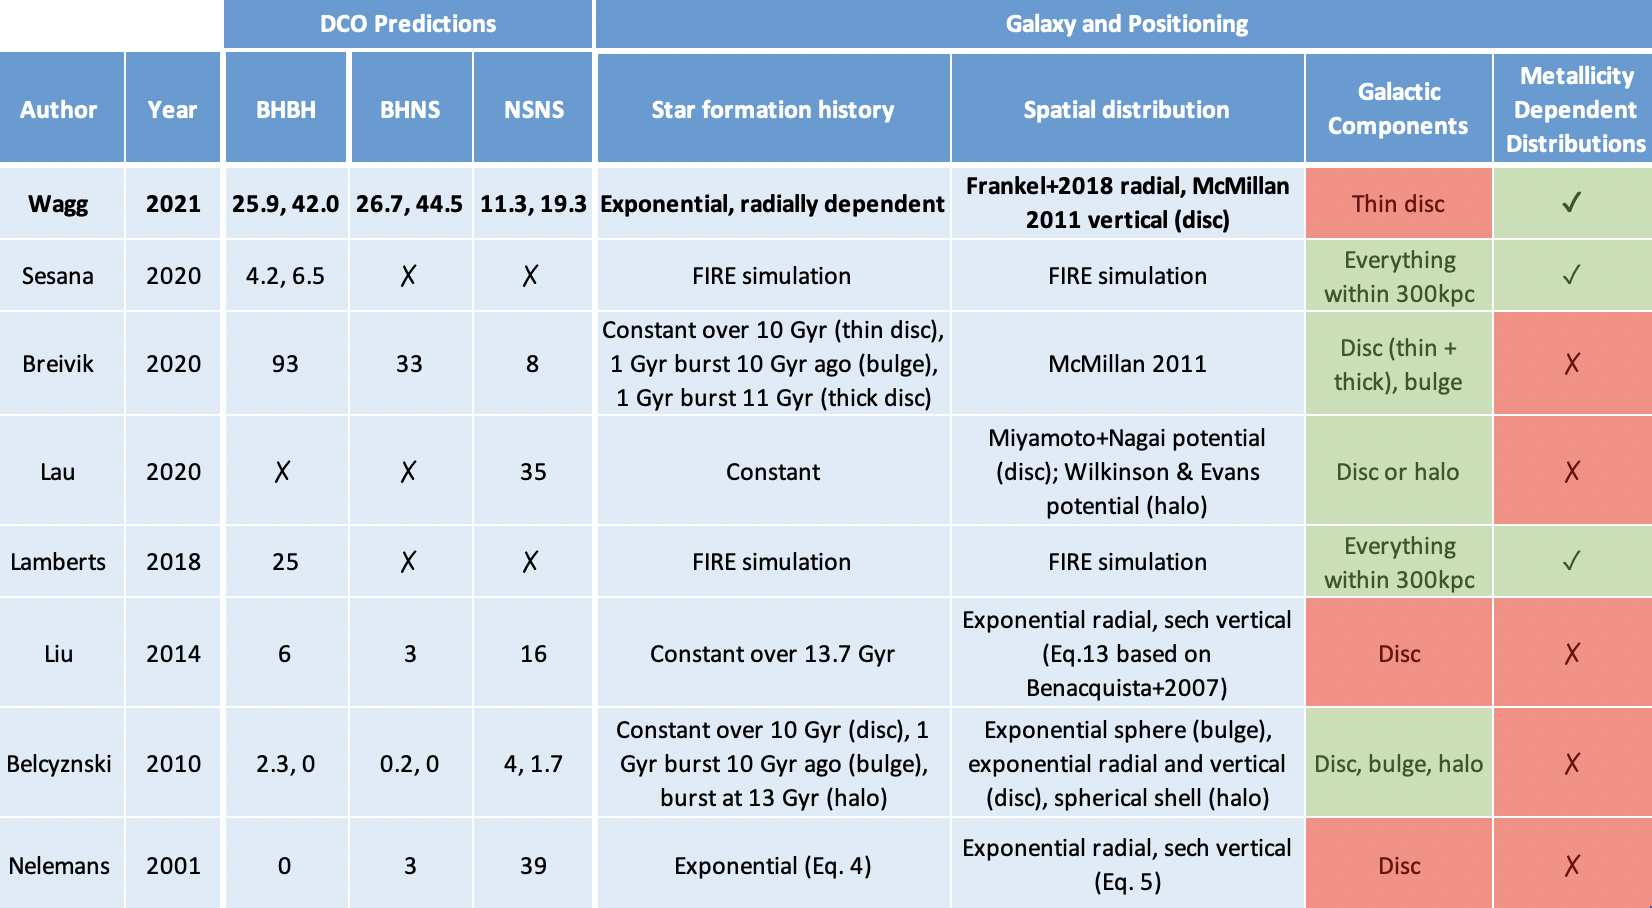
\includegraphics[width=\textwidth]{5_compare_dco_1.png}

    \vspace{0.5cm}

    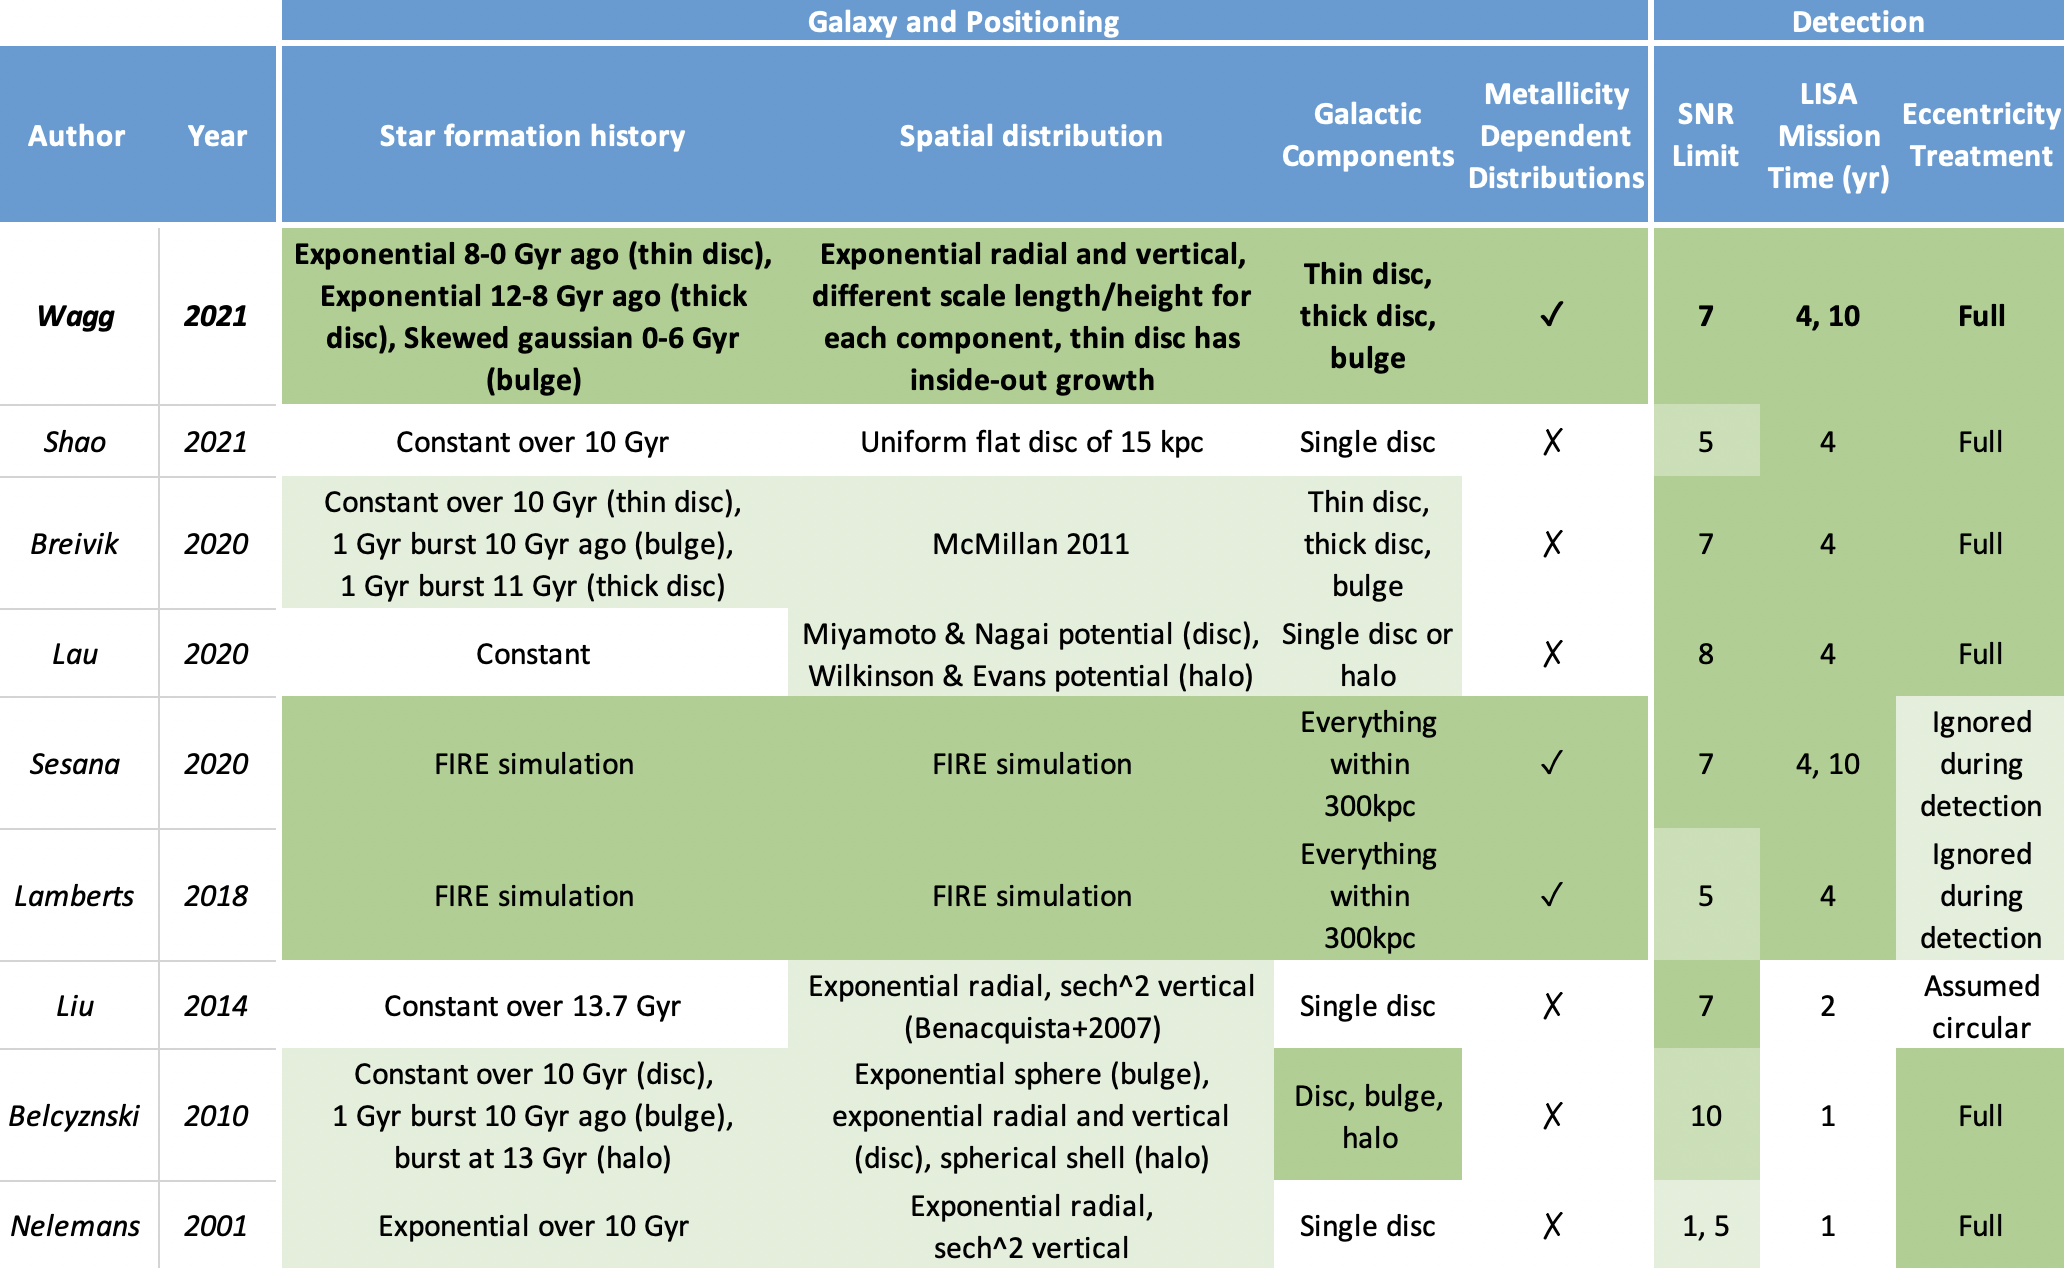
\includegraphics[width=\textwidth]{5_compare_dco_2.png}
    \caption{A table comparing previous studies of a similar nature to this work. The works listed in the table are \citet{Nelemans+2001,Belczynski+2010,Liu+2014,Lamberts+2018,Lau+2020,Breivik+2020,Sesana+2020}.}
    \label{fig:previous_studies}
\end{figure*}

In Figure~\ref{fig:previous_studies}, we compare similar previous studies that have investigated the population of stellar mass BHBHs, BHNSs and NSNSs that are detectable with LISA. The table details the expected detection rates predicted by each paper as well as their assumptions regarding their Milky Way galaxy model, binary population synthesis simulation and LISA mission specifications. This table not include the number papers on the LISA WDWD population as we do not make predictions for these DCOs. We additionally do not include papers that don't use population synthesis or do not simulate sources in the Galactic plane \citep[e.g.][]{Andrews+2020, Kremer+2018} such that we only compare with papers with similar methodology and focus.

\citet{Nelemans+2001} were the first to investigate the population of LISA detectable stellar mass double compact objects. Their predictions of the number of detectable DCOs are very different from our own, where we find a significantly higher detection rate for BHBHs and BHNSs, as well as a slightly lower rate for NSNSs. However, since the publication of their paper, there have been many changes both to the specifications of LISA (such as the mission length and SNR threshold for detection) and our understanding of massive star evolution, which strongly affect the expected detections rates.

\citet{Belczynski+2010} built upon this work by using a different population synthesis code with two model variations and a multi-component model for the Milky Way. They found a similar number of BHBH and BHNS detection to \citet{Nelemans+2001}, but a lower number of NSNS detections. The low total detection rate for all DCOs in this paper is unsurprising given the relatively high SNR threshold of 10 and short mission length of 1 year. The reduced mission length means that the source signal has much less time to accumulate, whilst also fewer WDWDs can be resolved in this time, leading to a weaker signal and an increased Galactic confusion noise relative to our work.

More recently, \citet{Lamberts+2018} presented a new approach to the problem by using the FIRE simulation \citep{Hopkins+2014} to distribute their sources rather than an analytical model of the Milky Way, thus being the first paper in this area to incorporate metallicity dependence into their Milky Way model. \citet{Sesana+2020} followed up on this paper using the same simulated BHBH population and presented updated results for the number of expected BHBH detections. They find significantly fewer BHBHs than our fiducial model despite using the same SNR threshold and LISA mission length.

The discrepancy between their results and ours could be a result of different implicit assumptions in their population synthesis code, however we expect that BSE should be similar to COMPAS since it provided the basis of the COMPAS code. Another major difference is that, unlike this work, they assume that all binaries are circular for the purpose of detection in LISA, which could result in a lower number of detections by missing eccentric binaries that appear as weaker signals when assumed to be circular. We also improve upon this work by using a larger number of metallicity bins since a low number of metallicity bins can produce artificial features in the mass distribution of DCOs and possibly affect the detection rate.

\citet{Lau+2020} focussed on the number of Galactic NSNS binaries that could be detected by LISA. Their study uses the same population synthesis code, COMPAS, as this work, though an earlier version. Despite this, their study found a much larger number of detections. They make several different physical assumptions in their population synthesis, using the \citet{Fryer+2012} \textit{rapid} remnant mass prescription, limiting the maximum neutron star mass to $2 \unit{M_{\odot}}$ and not implementing PISN. However, we note that none of these assumptions strongly affect the NSNS LISA detection rate (see bottom panel of Fig.\,\ref{fig:detection_rates}, models \modRapid{}, \modNSLow{} and \modNoPISN{}).

We therefore surmise that the difference between our results is likely due to way in which we simulate the Milky Way. \citet{Lau+2020} assumes constant star formation, solar metallicity and distributes binaries without any considerations of the chemical enrichment history of the Milky Way, whilst we use the distributions from \citet{Frankel+2018} for the star formation rate, metallicity and positions. The \citet{Frankel+2018} star formation rate decreases over time and the metallicity distribution peaks above solar metallicity, both changes that could decrease the NSNS detection rate given that we find most NSNS binaries in our sample have short inspiral times compared to the age of the Milky Way and higher metallicity would lead to increased stellar winds and hence less massive DCOs.

Finally, \citet{Breivik+2020} introduced the population synthesis code COSMIC and presented detections for many different DCO types in LISA using this code. They find that LISA will detect 93 BHBH, 33 BHNS and 8 NSNS binaries in the Milky Way over a 4 year mission. They make many different physical assumptions, the most notable being that \citet{Breivik+2020} assumes the optimistic CE scenario. Thus it would be more prudent to compare to our results from model \modOpt{} in which we find 118, 52 and 7 detections respectively. Thus the NSNS rate is consistent but we find higher rates for the BHBHs and BHNSs. These differences are likely due to using a different population synthesis code (COSMIC) and using a different model for the Milky Way, particularly the assumptions of two fixed metallicities.